\chapter{Tools \& Methods}

\section{Instrumentation}

\par As the atmosphere of the Earth is opaque to X-rays and gamma-rays, studying high-energy astrophysical phenomena requires the use of space-based observatories.  A number of satellites dedicated to the study of X-rays have been launched over the years, starting with \textit{UHURU} in 1970 \citep{Giacconi_Uhuru} and, most recently, \textit{Hitomi} in 2016 \citep{Takahashi_Hitomi}.  We use data from a number of these missions in the research reported in this thesis; in particular we use data from the NASA satellites\textit{RXTE}, \textit{Swift} and \textit{Chandra}, the European satellites \textit{XMM-Newton} and \textit{INTEGRAL}, and the Japanese satellite \textit{Suzaku}.  This section introduces the instruments used in my studies, as well as the tools used to extract their data for further analysis.

\subsection{The \textit{Rossi X-Ray Timing Experiment}}

\par The \textit{Rossi X-Ray Timing Experiment}, more commonly known as \textit{RXTE}, was a NASA-operated satellite launched from Cape Canaveral on December 30, 1995 \citep{Bradt_RXTE}.  \textit{RXTE} was primarily an X-ray observatory, constructed specifically to study X-ray QPOs seen in X-ray Binaries \citep{Bradt_XTEaims}.  The observatory operated until January 5, 2012, when it was decommissioned.
\par \textit{RXTE} contained three instruments.  The main instruments consisted of two X-ray telescopes: the Proportional Counter Array ('PCA', \citealp{Jahoda_PCA}) and the High Energy X-Ray Timing Experiment ('HEXTE' \citealp{Gruber_HEXTE}).  The satellite also carried an X-ray All-Sky Monitor (ASM, \citealp{Levine_ASM}).
\par PCA consisted of 5 Proportional Counting Units (PCUs) which were sensitive between $\sim2$--$60$\,keV.  The instrument had an excellent time resolution approaching 1\,$\mu$s, and an energy resolution of $\sim18\%$ at 6\,keV.  X-rays were guided onto the detectors by a collimator, resulting in an instrument field of view with a full-width half-maximum of 1$^\circ$.  There was a 6500\,cm$^2$ collecting area, and no angular resolution.
\par The HEXTE instrument provided complimentary coverage at higher energies, being sensitive between $\sim15$--$250$\,keV.  This instrument consisted 8 detectors, with a total collecting area of 1600\,cm$^2$, and had a similar field of view to that of PCA.  The time resolution is 8\,$\mu$s, and the energy resolution is 15\% at 60\,keV.
\par Finally, ASM was a soft X-ray all sky-monitor which covered 80\% of the sky every 90 minutes.  It was sensitive in the range 2--10\,keV, with a total collecting area of 90\,cm$^2$ and a spatial resolution of $3'\times15'$.  Due to its near continual coverage of the sky, ASM was excellent for long-term monitoring of transients in the soft X-ray sky.

\subsubsection{Data Formatting}

\par Much of the work in this thesis is based largely on data from PCA, which is freely available through the HEASARC archive maintained by NASA's Goddard Flight Centre\footnote{\url{https://heasarc.gsfc.nasa.gov/cgi-bin/W3Browse/w3browse.pl}}.  In PCA, as well as in other X-ray instruments, this data takes one of two forms:
\begin{itemize}
\item \textbf{Event-Mode Data:} A list of photon arrival times.  Depending on the instrument and observing mode, each of these times will have an associated channel, information about where in the detector the photon hit and a flag indicating the pattern that the photon made on the detector.
\item \textbf{Binned Data:} A list of evenly space time bins with the number of photons which arrived during each.  Depending on the instrument and observing mode, this may be accompanied by some information on the channel distribution of photons arriving in each bin.
\end{itemize}
\par The channel a photon falls into is denoted by its energy, although the channel-to-energy conversion for a particular instrument changes over time as the instrument degrades or settings are altered.  The channel-to-energy conversions for PCA can be found at \url{https://heasarc.gsfc.nasa.gov/docs/xte/e-c_table.html}.
\par Both event-mode and binned-mode data are stored in a Flexible Image Transit System (\texttt{.fits}) format.  This is a hierarchical data format consisting of a number of `Header Data Units' (HDUs), each of which contains data in some format and a header with details of the format.  In addition to either an event list or a table of binned data, these files also contain a list of Good Time Intervals (GTIs) during which the satellite was functioning normally, as well as an amount of housekeeping information such as the start and end times of the observation.
\par For PCA observations of faint objects, event mode data with full energy information (referred to as \texttt{goodxenon}-mode data) is generally available.  However when brighter objects were observed, telemetry constraints sometimes prevented this full information from being transmitted to Earth.  In this case, a number of data products are available; \texttt{Standard1} data (binned data with 0.125\,s time resolution but no energy information), \texttt{Standard2} data (binned data with 16\,s time resolution, divided into 128 bins by channel) and a number of other data products with various time and energy resolutions.  While \texttt{Standard2} data is useful for studying spectral variability over long timescales, it is not useful for studying the second-to-minute scale variability reported on in this thesis.  We used \texttt{goodxenon} data when available, as this allowed us to use the maximum possible time and energy resolutions, and various other datamodes including \texttt{Standard1} when \texttt{goodxenon} mode data was not available.

\subsubsection{Data Extraction}

\par To perform science with PCA or other instruments, we must extract science products (such as lightcurves, power spectra and energy spectra) from the raw data.  Tools to create lightcurves and power spectra from PCA data are available as part of \texttt{FTOOLS} \footnote{\url{https://heasarc.gsfc.nasa.gov/ftools/}}, a free NASA-maintained suite of software for manipulating \texttt{.fits} formatted data.  I also wrote my own software \texttt{PANTHEON} (\citealp{Court_PANTHEON}, presented in Appendix \ref{app:PAN}) to extract a number of additional products, such as power spectra and spectrograms.

\subsubsection{Background Correction}

\subsection{The \textit{Neil Gehrels Swift Observatory}}

\subsection{\textit{XMM-Newton}}

\subsection{\textit{Chandra}}

\subsection{\textit{Suzaku}}

\subsection{\textit{NuStar}}

\subsection{\textit{INTEGRAL}}

\section{Raw Data Extraction}

\section{Lightcurve Analysis}

\subsection{Flare-Finding Algorithm}
\label{sec:Flares}

\par The algorithm used to find flares is performed as such (see also Figure \ref{fig:BurstAlg}):

\begin{enumerate}
  \item Choose some threshold values $T_L$ and $T_H$.  Set the value of all datapoints below $T_L$ to zero.
  \item Retrieve the x-co-ordinate of the highest value remaining in the dataset.  Call this value $x_m$ and store it in a list.
  \item Set the value of point at $x_m$ to zero.
  \item Scan forwards from $x_m$.  If the selected point has a nonzero value, set it to zero and move to the next point.  If the selected point has a zero value, move to step (v).
  \item Scan backwards from $x_m$.  If the selected point has a nonzero value, set it to zero and move to the previous point.  If the selected point has a zero value, move to step (vi).
  \item Retrieve the y-co-ordinate of the highest value remaining in the dataset.  Call this $y_m$.
  \item If $y_m>T_H$, repeat steps (ii)--(vi).  If $y_m<T_H$, proceed to step (viii).
  \item Restore the original dataset.
  \item Retrieve the list of $x_m$ values found in step (ii).  Sort them in order of size.
  \item For each pair of adjacent $x_m$ values, find the x-coordinate of the datapoint between them with the lowest y-value.  Call these values $x_c$.
  \item This list of $x_c$ can now be used to demarcate the border between peaks.
\end{enumerate}

\begin{figure}
    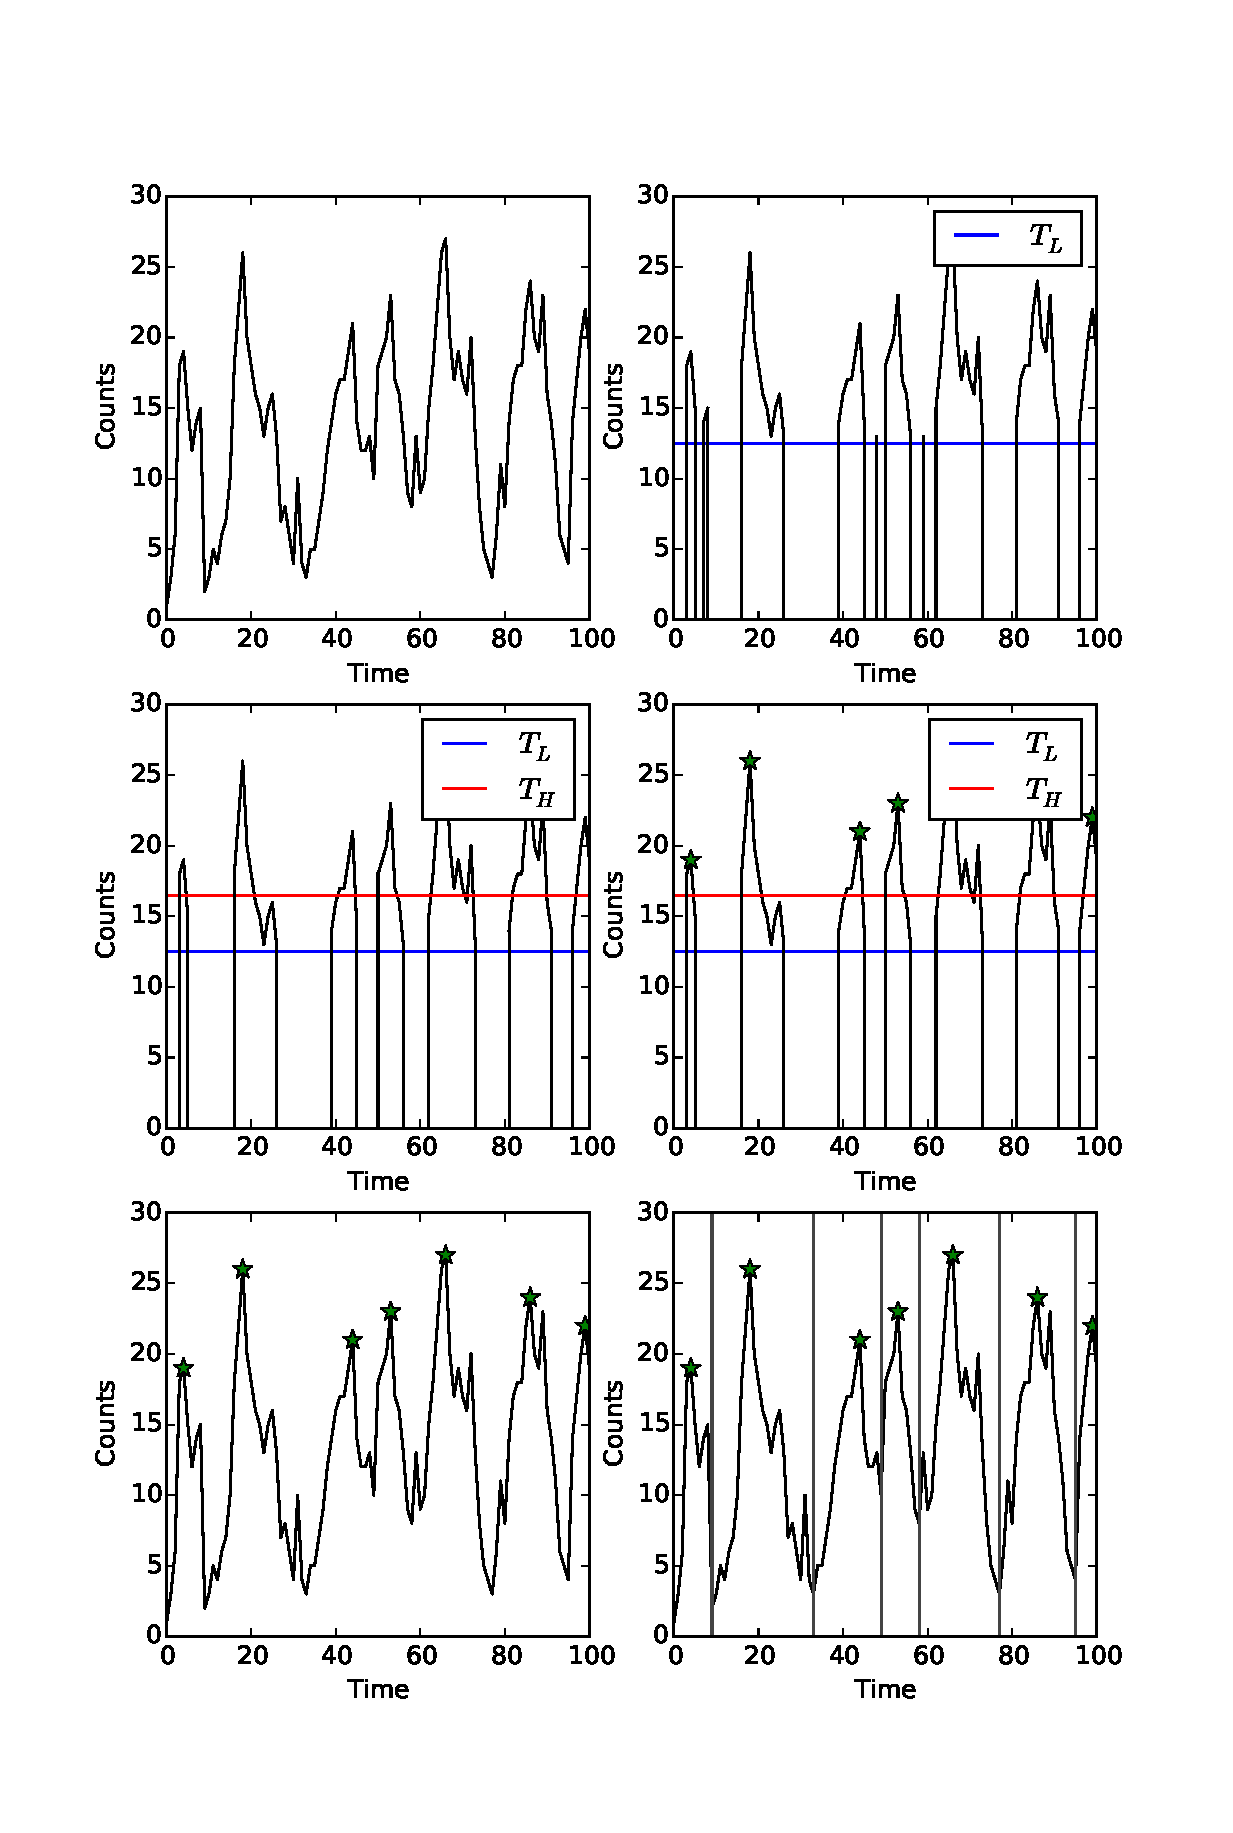
\includegraphics[width=\columnwidth, trim = 0mm 30mm 0mm 28mm]{images/steps.eps}
    \captionsetup{singlelinecheck=off}
    \caption{From top-left: (i) An untouched data-set.  (ii) The dataset with all $y<T_L$ removed.  (iii) The dataset with all contiguous nonzero regions with $\max(y)<T_H$ removed.  (iv) The peak x-values $x_m$.  (v) The restored dataset with the peak x-values $x_m$ highlighted.  (vi) The boundaries between adjacent peaks.}
   \label{fig:BurstAlg}
\end{figure}

The values $T_L$ and $T_H$ can also be procedurally generated for a given piece of data:

\begin{enumerate}
  \item Select a small section of the dataset or a similar dataset (containing $\sim20$ peaks by eye) and note the location $x_e$ of all peaks found by eye.
  \item Let $P_L$ and $P_H$ be two arbitrary values in the range $[0,100]$.
  \item Let $T_L$ ($T_H$) be the $P_L$th ($P_H$th) percentile of the y-values of the subsection of dataset.
  \item Run the flare-finding algorithm up to step (ix).  Save the list of $x_m$.
  \item Split the dataset into bins on the x-axis such as the bin width $b\ll p$, where $p$ is the rough x-axis separation between peaks.
  \item For each bin, note if you found any value in $x_m$ falls in the bin and note if any value of $x_e$ falls in the bin.
  \item Using each bin as a trial, compute the Heidke Skill Score \citep{Heidke_SKSC} of the algorithm with the method of finding peaks by eye:
  \begin{equation}HSS = \frac{2(AD-BC)}{(A+B)(B+D)+(A+C)(C+D)}
  \label{eq:HSS}
  \end{equation}
  Where $A$ is the number of bins that contain both $x_e$ and $x_m$, $B$ ($C$) is the number of bins that contain only $x_m$ ($x_e$) and $D$ is the number of bins which contain neither \citep{Kok_YesNo}.
  \item Repeat steps (iii)--(vii) for all values of $P_H>P_L$ for $P_L$ and $P_H$ in $[1,100]$.  Use a sensible value for the resolution of $P_L$ and $P_H$.  Save the HSS for each pair of values
  \item Locate the maximum value of HSS, and note the $P_L$ and $P_H$ values used to generate it.  Use these values to generate your final $T_L$ and $T_H$ values.
\end{enumerate}

We show an example of Heidke skill score grid for this algorithm, applied to a Class IV observation, in Figure \ref{fig:Heidke}.

\begin{figure}
    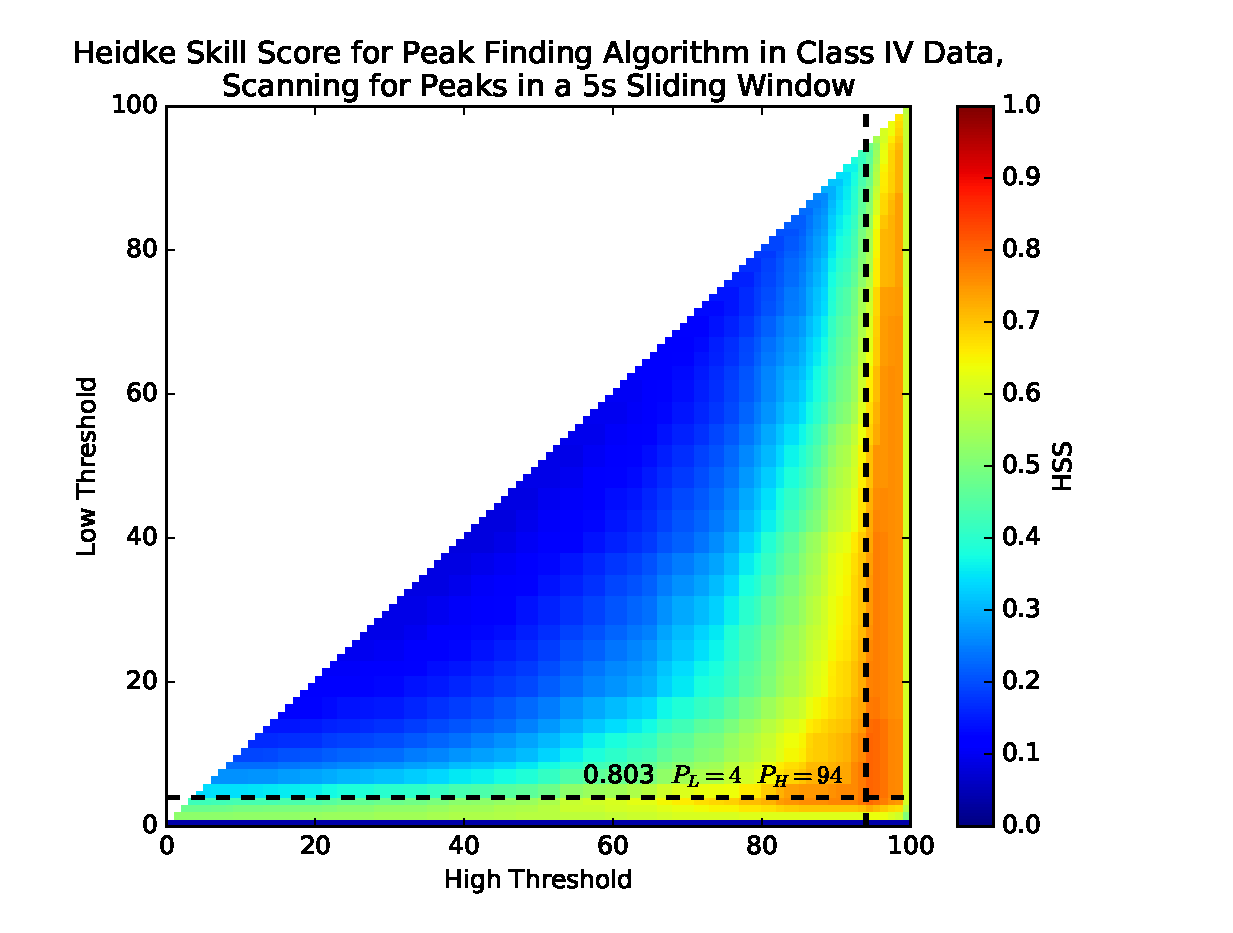
\includegraphics[width=\columnwidth, trim = 0mm 10mm 0mm 10mm]{images/HSS_J.eps}
    \captionsetup{singlelinecheck=off}
    \caption{The Heidke Skill score of a Class IV observation of IGR J17091-3624 for a selection of different values $P_L$ and $P_H$.}
   \label{fig:Heidke}
\end{figure}

\section{Timing Analysis}

\section{Spectral Analysis}

\subsection{Phase-Resolved Spectroscopy}
\label{sec:phasresspec}

